\section{Data Mining}
\label{dm}
Die vorliegende wissenschaftliche Fragestellung bewegt sich im Bereich des Data Minings. Das folgenden Kapitel soll dem Leser dazu eine Einführung in die Thematik geben, um ein grundlegendes Verständnis der Begriffe und Ziele des Data Minings zu erlangen\vref{defdm}. Darüber hinaus werden die Prozesse des Data Minings \vref{prozdm} beleuchtet, wobei der \textit{Knowledge Discovery in Data} Prozess -- methodischer Aufbau der späteren Umsetzung -- in \vref{kdd} nochmal ausführlich eruiert wird.

\subsection{Definition des Data Minings}
\label{defdm}

Der Bergriff des Data Minings reicht zurück bis in die 80er Jahre des letzten Jahrhunderts und verfolgt das Ziel, Wissen aus riesigen Datenmengen zu extrahieren.\seFootcite{Vgl.}{S.2}{Runkler.2015} Als ein Prozess des \textit{Sammelns, Säuberns, Verarbeitens und Analysierens von Daten, zur Gewinnung von nützlichen Informationen}\seFootcite{Vgl.}{S.1}{Aggarwal.2015} beschreibt Aggarwal diesen Begriff. Denn der immense Datenanstieg in den letzten Jahrzehnten erlaubt uns nicht einfach wertvolle Informationen oder organisiertes Wissen automatisch zu verstehen oder zu entnehmen. Das heutige \glqq Informationszeitalter\grqq~führte zum Beginn des renommierten Wissenschaftsbereich des Data Minings, der in der Literatur auch als natürliche Evolution der Informationstechnologie bezeichnet wird.\seFootcite{Vgl.}{S.1}{Garcia.2015}\seFootcite{Vgl.}{S.2}{Han.2012} Grundlegende interdisziplinäre, wissenschaftliche Teilgebiete des Data Minings sind, z.B. Statistik, maschinelles Lernen, Mustererkennung, Systemtheorie oder künstliche Intelligenz.\seFootcite{Vgl.}{S.2}{Runkler.2015}\seFootcite{Vgl.}{S.1}{Shi.2015}


Cleve und Han vergleichen die Suche nach Muster und Zusammenhänge in den Daten mit dem Abbau von Rohstoffen.\footnote{Die englische Übersetzung lautet \textit{\glqq Mining\grqq}} Sowie im Bergbau nach Schätzen wie Gold und Silber im Gestein sucht wird, so strebt das \gls{dm} nach dem Ableiten von Wissen aus den (Roh-)Daten.\seFootcite{Vgl.}{S.1}{Cleve.2014}\seFootcite{Vgl.}{S.5-6}{Han.2012} Ha9n geht sogar einen Schritt weiter und präferiert den Begriff des \textit{knowledge mining from data} -- referenzierend auf den verwendenden Terminus des \textit{gold mining} statt des \textit{rock or sand mining} -- da diese Bezeichnung das eigentliche Ziel der Gewinnung von Wissen beinhaltet.\seFootcite{Vgl.}{S.5-6}{Han.2012}\footnote{Weitere Termini nach Han: \textit{knowledge mining from data, knowledge extraction, data/pattern analysis, data archaeology, and data dredging.}}

\glqq Unter Wissen verstehen wir interessante Muster, die allgemein gültig sind, nicht trivial, neu, nützlich und verständlich.\grqq\seFootcite{Vgl.}{S.2}{Runkler.2015} Insofern wird das Ziel verfolgt komplexe Paradigmen zu erkennen, die durch die blanke Betrachtung der Daten nicht aufgedeckt werden könnten. Oftmals fehlt dem Datenanalyst das spezifische Fachwissen zur Erkennung von Mustern, sodass durch die Einbeziehung von Experten ein iterativer Prozess entsteht, bis ein gewünschtes Ergebnis erzielt wird. Zunächst werden aus den Daten, Informationen gewonnen, aus welchen wiederum das Wissen abgeleitet werden kann, wobei in diesem Prozess der Wissensextraktion die Datenmenge sukzessive abnimmt und sich verdichtet, wie in \vref{wissenprozess} verdeutlicht.

\begin{figure}[H]
\centering
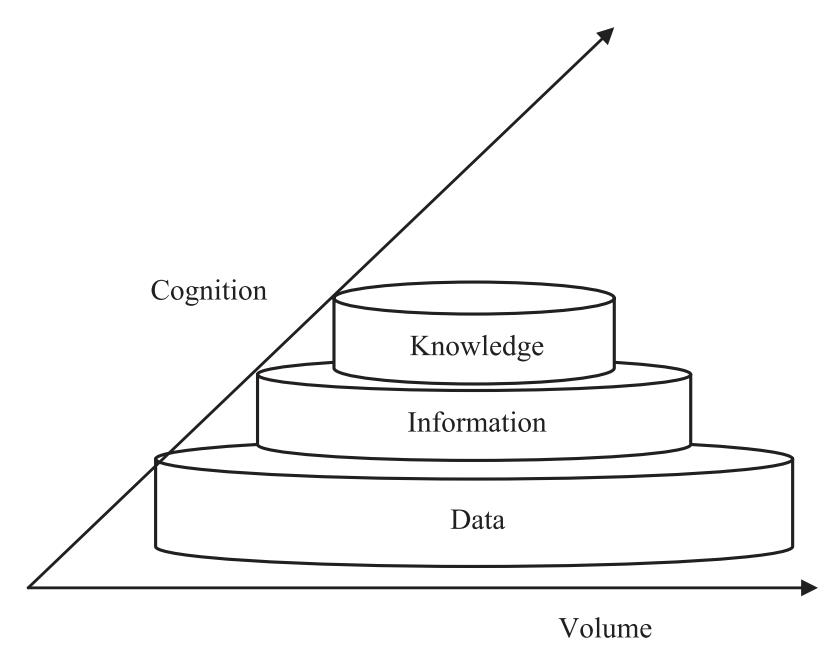
\includegraphics[scale=1.3]{se-wa-jpg/wissenprozess}
\caption[Wissensextraktion aus Daten]{Wissensextraktion aus Daten\protect\footnotemark}
\label{wissenprozess}
\end{figure}
\footnotetext{Vgl. Abbildung \textit{Shi} et al., Intelligent Knowledge, 2015, S.5}


Durch den Einsatz von modernster Computerhard- als auch software ist es möglich immens große Datenmenge zu erheben, zu verarbeiten und zu analysieren, wodurch in diesem Kontext der Begriff \textit{Big Data} entstanden ist.\seFootcite{Vgl.}{S.3}{Witten.2011} Big Data bezeichnet Datenmengen, die mit herkömmlichen Analysemethoden nicht mehr zu verarbeiten werden und den Einsatz von Data Mining benötigen.\seFootcite{Vgl.}{S.5}{Fasel.2016}\seFootcite{Vgl.}{S.1}{Shi.2015} Dazu ein paar ausgewählte Bespiele aus verschiedenen Datenbereichsquellen:\seFootcite{Vgl.}{S.2}{Aggarwal.2015}

\begin{itemize}
\item \textbf{Word Wide Web:} Die Anzahl der Dokumente im Internet hat schon lange die Milliarden Marke geknackt, wobei die des unsichtbaren Webs noch viel größer ist. Durch Nutzerzugriffe auf Inhalte werden auf Serverseite Log-Dateien kreiert, um beispielsweise die Auslastung und Zugangszeiten zu protokollieren. Andererseits wird das Kundenverhalten auf kommerziellen Seiten aufgezeichnet, um personalisierte Werbung schalten zu können.
\item \textbf{Benutzerinteraktion:} Festnetzanbieter nutzen die durch Telefonate entstanden Daten, wie Gesprächslänge und Ort, um relevante Muster über die Netzwerkauslastung, zielgerichtete Werbung oder auch anzusetzende Preise durch Datenanalyse zu extrahieren.
\item \textbf{Internet of Things:} Durch kostengünstige (tragbare) Sensoren und deren kommunikative Vernetzung entstand das \gls{iot}. Einer der Trends der heutigen Informationstechnologie, der durch die Erhebung von Massendaten eine signifikante Rolle für das Data Mining einnimmt.
\item \textbf{Weitere Beispiele:}  Social Media Plattformen (allen voran Facebook, Twitter und Co.), Finanzmärkte (z.B. der Aktienmarkt), Sport (z.B. Baseball, Basketball, Football oder wie in dieser Arbeit Fußball), uvm.\seFootcite{Vgl.}{S.39}{Fayyad.1996}\seFootcite{Vgl.}{S.1-2}{Han.2012}
\end{itemize}

Wir befinden uns in einer Situation, in der wir reich an Daten sind, jedoch arm an Informationen und Wissen. Der unglaubliche rasante und gigantische Datenzuwachs hat bei langem unsere menschliche Vorstellungskraft und Möglichkeiten übertroffen, sodass wir auf mächtige Werkzeuge angewiesen sind.(siehe \vref{dmmethoden}) Die sich immer weiter ausbreitende Lücke zwischen Daten und Information führt nur durch die Nutzung von Methoden des Data Minings zu den \glqq \textit{Golden Nuggets of Knowledge}\grqq.\seFootcite{Vgl.}{S.5}{Han.2012} Dazu müssen die (Roh-)Daten gezielt ausgewählt und umstrukturiert werden, um diese anschließend von Algorithmen analysieren zu können. Folglich entstanden Data Mining Prozesse, die dieses Problem mit Hilfe systematischer Abläufe lösen sollen.(vgl. \vref{prozdm}) Zudem wird \glqq Data Mining [...] heute durch eine zunehmende Anzahl von Software-Tools unterstützt, z. B. KNIME, MATLAB, SPSS, SAS, STATISTICA, TIBCO Spotfire, R, Rapid Miner, Tableau, QlikView, oder WEKA.\grqq\seFootcite{Vgl.}{S.3}{Runkler.2015} Das Software-Tool \textit{MatLab} wird innerhalb der Funktionsmodellierung in \vref{fm} vorgestellt und anschließend als Werkzeug zur Nutzung von Data Mining Methoden in der Umsetzungsphase genutzt.(vgl. \vref{umsetzung})


\subsection{Data Mining Prozesse}
\label{prozdm}

In der Literatur dis\-tin\-guie\-ren viele Wissenschaftler den Begriff des eigentlichen Data Minings, gegenüber dem Gesamtprozess der Extraktion von Wissen. Andere wiederum behandeln beide Termini synonym zu einander.\seFootcite{Vgl.}{S.39}{Fayyad.1996}\seFootcite{Vgl.}{S.2}{Mariscal.2010}\seFootcite{Vgl.}{S.1}{Garcia.2015} Schlechte Qualität der Daten mindert die Leistungsfähigkeit des Data Minings. Um die Aussagekraft der Daten nicht zu gefährden, sind vorab Prozessschritte notwendig, die Daten in geeigneter Form für die Methoden des Data Minings bereitstellen.\seFootcite{Vgl.}{S.10}{Garcia.2015}  Hierzu werden im folgenden kurz die zwei bekanntesten Prozessmodelle vorgestellt:

\begin{itemize}
\item \gls{kdd}
\item \gls{crisp-dm}
\end{itemize}

\subsubsection{Knowledge Discovery in Data}
\label{dmkdd}

Der Begriff des \textit{Knowledge Discovery in Data} Prozesses wurde in den frühen 90er Jahren geprägt und wird als \glqq nicht trivialer Prozess zur Identifizierung von gültigen, neuartigen, potentiell sinnvolle und letztlich verständlichen Muster in Daten\grqq\seFootcite{Vgl.}{S.1-2}{Garcia.2015}\seFootcite{Vgl.}{S.41}{Fayyad.1996} definiert.\seFootcite{Vgl.}{S.2}{Mariscal.2010} Erstmals wurde der Terminus von Gregory Piatetsky-Shapiro auf der \textit{International Joint Conference on Artificial Intelligence}, 1989 in Detroit (USA), formuliert und vorgestellt.\seFootcite{Vgl.}{S.1}{Adhikari.2015} Der in \vref{kddpic} abgebildete iterative \gls{kdd}-Prozess nach Fayyad beinhaltet folgende Schritte, wobei das \gls{dm} als ein eigener Prozessschritt ausgewiesen wird:\seFootcite{Vgl.}{S.5}{Cleve.2014}

\begin{itemize}
\item \textbf{Datenselektion}: Auswahl der geeigneten Datenmengen
\item \textbf{Datenvorverarbeitung}: Behandlung fehlender oder problembehafteter Daten
\item \textbf{Datentransformation}: Umwandlung in adäquate Datenformate
\item \textbf{Data Mining}: Suche nach Muster
\item \textbf{Interpretation und Evaluation}: Interpretation der Ergebnisse und Auswertung
\end{itemize}

Auf die einzelnen Prozessschritte und deren Methoden wird genauer in \vref{kdd} eingegangen. 
\begin{figure}[H]
\centering
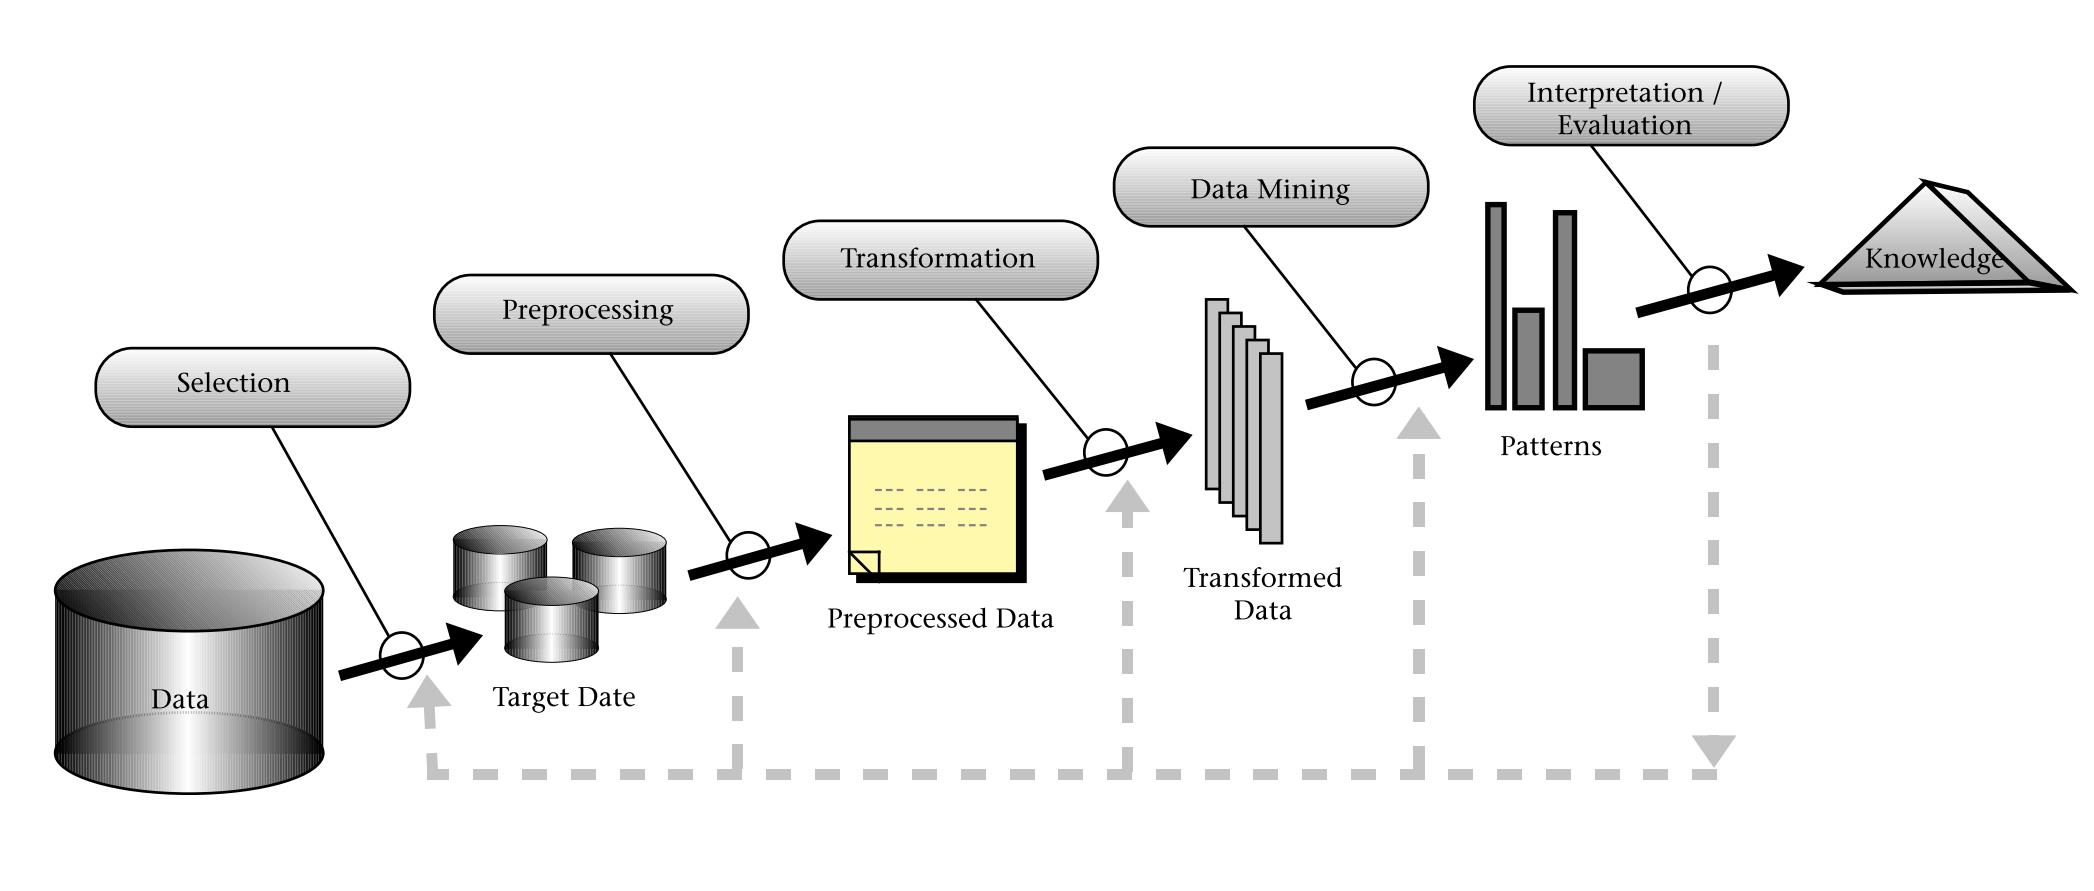
\includegraphics[scale=0.85]{se-wa-jpg/kdd}
\caption[Der Knowledge Discovery in Data Prozess]{Der Knowledge Discovery in Data Prozess\protect\footnotemark}
\label{kddpic}
\end{figure}
\footnotetext{Vgl. Abbildung \textit{Fayyad} et al., From Data Mining to Knowledge, 1996, S.41}


\subsubsection{CRISP-DM}
Das \gls{crisp-dm}-Modell wurde im Jahr 200 durch ein Konsortium, bestehend aus mehreren Firmen, entwickelt. Beteiligt waren daran:\seFootcite{Vgl.}{S.6}{Cleve.2014}\seFootcite{Vgl.}{S.3}{Mariscal.2010}

\begin{itemize}
\item NRC Corporation,
\item Daimler AG,
\item SPSS,
\item Teradata und
\item OHRA.
\end{itemize}

Dieses Modell verfolgt das Ziel, einen standardisierten und branchenübergreifenden Data Mining Prozess zu definieren und das dadurch berechnete Modell zu validieren. Hierbei wird von einem Lebenszyklus mit den folgenden sechs Etappen ausgegangen, die in \vref{crisp} dargestellt werden.\seFootcite{Vgl.}{S.6-8}{Cleve.2014}

\begin{figure}[H]
\centering
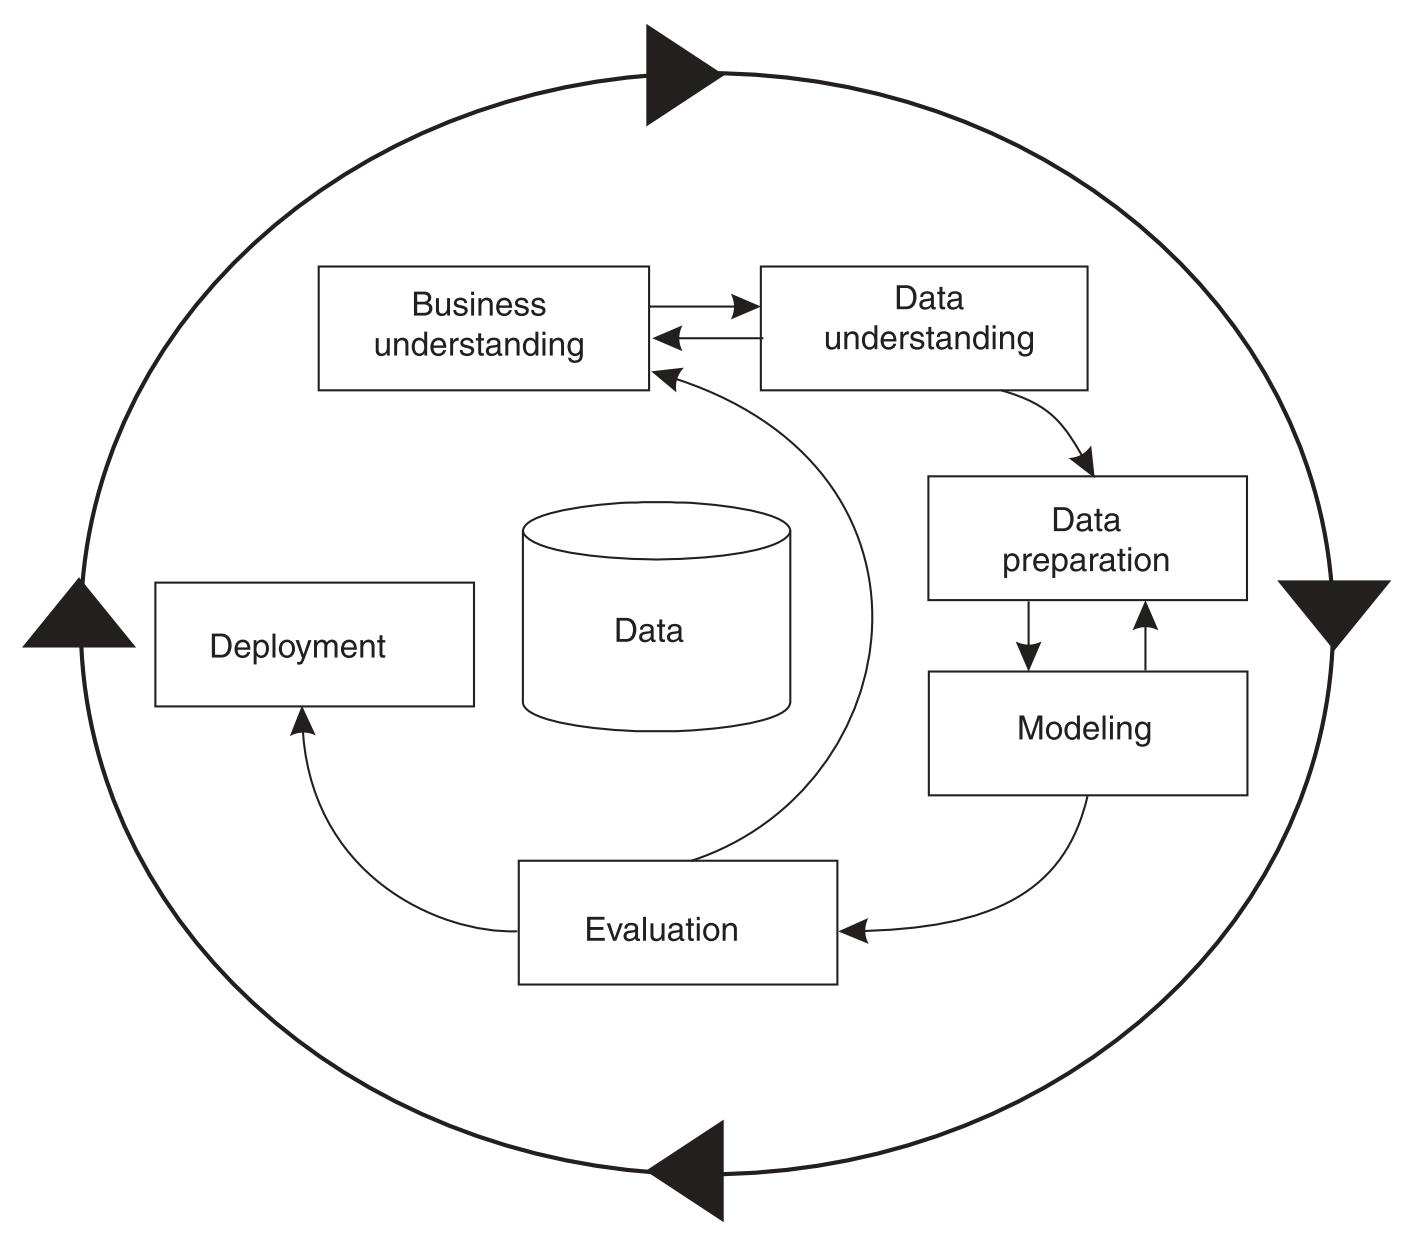
\includegraphics[scale=0.7]{se-wa-jpg/crisp}
\caption[CRISP-DM Prozess]{CRISP-DM Prozess\protect\footnotemark}
\label{crisp}
\end{figure}
\footnotetext{Vgl. Abbildung \textit{Mariscal} et al., A survey of data mining, 2010, S.13}


\paragraph{Verstehen der Aufgabe}
Hier steht das grundsätzliche Verständnis des Fachgebiets und der Aufgabe im Vordergrund. Die Ziele werden abgestimmt, Ressourcen des Unternehmens ermittelt und die Ausgangssituation bestimmt. Weiterhin müssen Erfolgskriterien und Risiken quantifiziert werden, um eine Kostenplanung aufstellen zu können. 
\paragraph{Verständnis der Daten}
Die Phase beschäftigt sich mit den benötigten Daten für das Ziel der Analyse. Daten werden gesammelt und beschrieben, um deren betriebliche Bedeutung zu verstehen.
\paragraph{Datenvorbereitung}
Es gilt den Data Mining Schritt vorzubereiten, wobei fehlerhafte und inkonsistente Daten korrigiert werden müssen, um diese schließlich in eine Datenstruktur zu transformieren, die für die Methoden des Data Minings nutzbar sind.
\paragraph{Data Mining - Modellbildung}
In dieser Phase wird ein Modell mit Hilfe des Data Minings erstellt, welches durch ein iteratives Verfahren immer wieder verfeinert und verbessert wird. 
\paragraph{Evalution}
Die erzielten Ergebnisse werden mit den aus Phase 1 erstellten Erfolgskriterien gemessen, um beispielsweise festzustellen, ob der wirtschaftliche Nutze erzielt wurde.
\paragraph{Einsatz im Unternehmen}
Zuletzt wird der Einsatz der Resultate in das Unternehmen vorzubereiten und in das operative Geschäft zu integrieren.

Das Modell bezieht und orientiert sich, wie schon im Namen zu lesen, stark an wirtschaftlichen Projekten und beschreibt \textit{was} zu tun ist, aber nicht genau \textit{wie}, sodass Projektteams innerhalb dieses Rahmens beginnen ihre eigenen Methoden zu verwenden.\seFootcite{Vgl.}{S.4}{Mariscal.2010}

Im Vergleich zum \gls{kdd}-Modell nach Fayyad, sind die Phase 1 und 2 des \gls{crisp-dm}-Modells sehr stark projektabhängig und spiegeln die Sicht der Industrie auf das Projekt wider.\seFootcite{Vgl.}{S.8}{Cleve.2014} Im Gegensatz dazu konzentriert sich der \gls{kdd}-Prozess auf die Datenbereitstellung und Analyse, sodass dieser als grundlegende Methodik für die spätere Umsetzung der wissenschaftlichen Aufgabenstellung herangezogen wird und genauer in \vref{kdd} durchleuchtet wird.

Mariscal et al. diskutieren in ihrer Studie weitere zahlreiche Prozessmodelle zur Extraktion von Wissen aus riesigen Datenmengen, wobei die Kernelemente der Datenselektion, -vorverarbeitung und -tranformation, sowie der anschließende Schritt des eigentlichen Data Minings immer wieder aufzufinden sind.\seFootcite{Vgl. vorgestellte Modelle}{}{Mariscal.2010} Nicht zuletzt sei zu erwähnen, dass in der Literatur unterschiedliche Auffassungen zu dem Begriff \textit{Data Mining} existieren und dieser oftmals mit den Data Mining Prozessen synonym verwendet wird. Ein Hinweis darauf sind auch die weit über 500 wissenschaftliche Artikel zu dem Journal \textit{Data Mining and Knowledge Discovery} auf Springer Link.

